\begin{figure*}[!t]
  \centering
  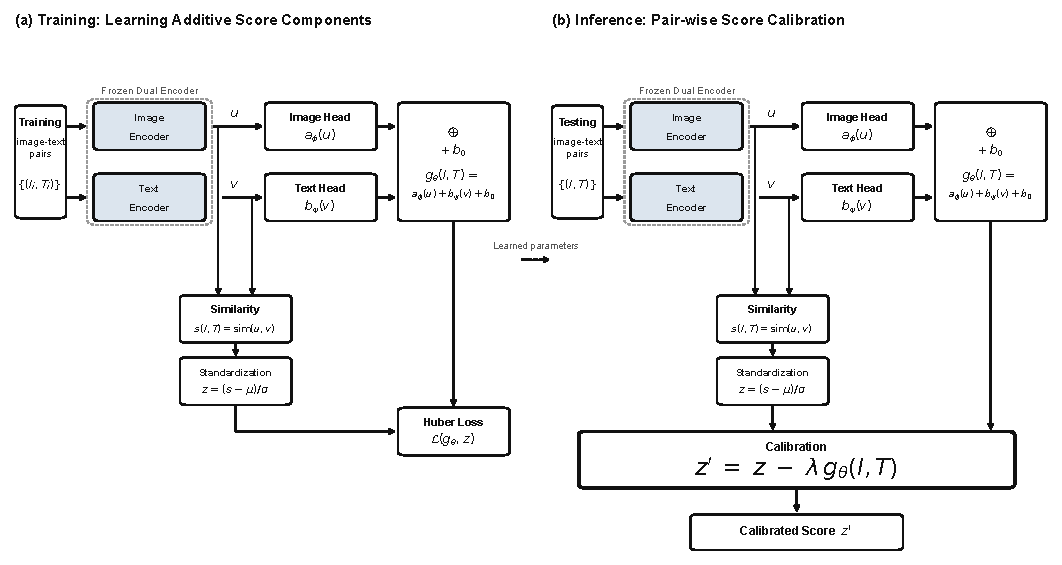
\includegraphics[width=0.88\textwidth]{fig2_crd.pdf}
  \caption{Overview of the proposed CRD framework. (a) During training, CRD
  learns additive image-conditioned and text-conditioned score components from
  row-level standardised image--text similarity scores. Both encoders are frozen
  and only the two heads and the bias $b_0$ are optimised. (b) During inference,
  the estimated additive component is subtracted from the raw standardised
  similarity to obtain a calibrated pair-wise score. The heads and the statistics
  $\mu,\sigma$ are fixed from training and $\lambda$ is chosen on a validation
  split; a single pair is sufficient and no reference bank or cycle is used.}
  \label{fig:overview}
\end{figure*}
